\section{Homepage}

The homepage (shown below in \ref{fig:TAHomepage}) is implemented with the code shown at the bottom of this section.

\begin{figure}[h]
\centering
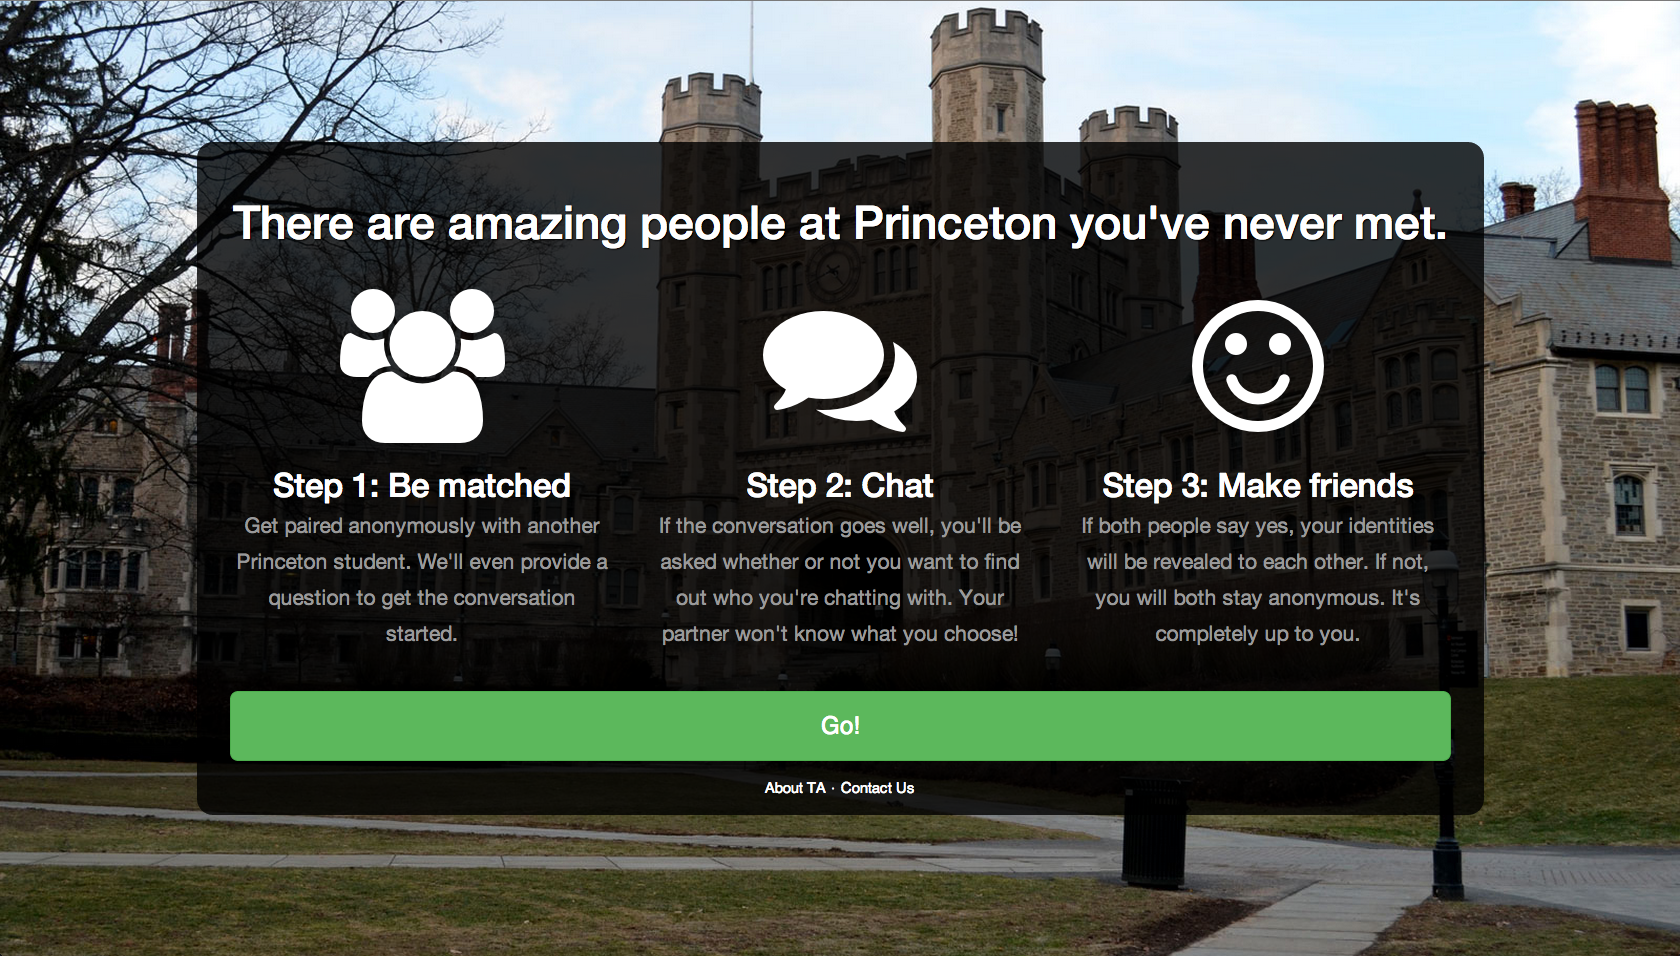
\includegraphics[trim= 35mm 0mm 35mm 0mm, clip, scale=0.25]{./Figures/TAHomepage}
\caption{Tigers Anonymous Homepage}
\label{fig:TAHomepage}
\end{figure}

\lstset{language=HTML}
\begin{lstlisting}

<!DOCTYPE html>
<html>
  <head prefix="og: http://ogp.me/ns#">
    <title>Tigers Anonymous</title>
    <link rel="icon" href="img/favicon.ico" type="image/x-icon">
    <meta name="viewport" content="width=device-width, initial-scale=1.0, user-scalable=no">
    <meta property="og:title" content="Tigers Anonymous">
    <meta property="og:description" content="There are amazing people at Princeton you've never met.">
    <meta property="og:url" content="http://www.tigersanonymous.com">
    <meta property="og:image" content="http://www.tigersanonymous.com/img/ta1024.png">
    <meta property="og:image:type" content="image/png">
    <meta property="og:image:width" content="1024">
    <meta property="og:image:height" content="1024">
    <link rel="stylesheet" href="//netdna.bootstrapcdn.com/bootstrap/3.0.3/css/bootstrap.min.css">
    <link href="//netdna.bootstrapcdn.com/font-awesome/4.0.3/css/font-awesome.css" rel="stylesheet">
    <link href="css/index.css" rel="stylesheet" type="text/css" media="all">
    <script>
      (function(i,s,o,g,r,a,m){i['GoogleAnalyticsObject']=r;i[r]=i[r]||function(){
      (i[r].q=i[r].q||[]).push(arguments)},i[r].l=1*new Date();a=s.createElement(o),
      m=s.getElementsByTagName(o)[0];a.async=1;a.src=g;m.parentNode.insertBefore(a,m)
      })(window,document,'script','//www.google-analytics.com/analytics.js','ga');
      ga('create', 'UA-23357698-2', 'tigersanonymous.com');
      ga('send', 'pageview');
    </script>
  </head>
  <body class="cover">
    <div class="wrapper">
      <div class="container">
        <div class="row text-center">
          <div class="col-md-12">
            <h1 class="hook">There are amazing people at Princeton you've never met.</h1>
          </div>
        </div>
        <div class="row how-it-works">
          <div class="col-md-4">
            <div class="row text-center padded-icon">
              <i class="fa fa-users large-icon"></i>
            </div>
            <div class="row text-center padded-text">
              <h2>
                Step 1: Be matched<br>
                <small>Get paired anonymously with another Princeton student. We'll even provide a question to get the conversation started.</small>
              </h2>
            </div>
          </div>
          <div class="col-md-4">
            <div class="row text-center padded-icon">
              <i class="fa fa-comments large-icon"></i>
            </div>
            <div class="row text-center padded-text">
              <h2>
                Step 2: Chat<br>
                <small>If the conversation goes well, you'll be asked whether or not you want to find out who you're chatting with. Your partner won't know what you choose!</small>
              </h2>
            </div>
          </div>
          <div class="col-md-4">
            <div class="row text-center padded-icon">
              <i class="fa fa-smile-o large-icon"></i>
            </div>
            <div class="row text-center padded-text">
              <h2>
                Step 3: Make friends<br>
                <small>If both people say yes, your identities will be revealed to each other. If not, you will both stay anonymous. It's completely up to you.</small>
              </h2>
            </div>
          </div>
        </div>
        <div class="row">
          <div class="col-md-12">
            <a href="/chat" class="go-btn btn btn-success btn-xlg btn-block">Go!</a>
          </div>
        </div>
        <div class="row text-center">
          <div class="col-md-12 footer">
            <a href="/about">About TA </a>
            &#8901;
            <a href="mailto:originblack609@gmail.com"> Contact Us</a>
          </div>
        </div>
      </div>
    </div>
  </body>
</html>

\end{lstlisting}

\section{About Page}

The About page (shown below in \ref{fig:TAAbout}) is implemented with the code shown at the bottom of this section.

\begin{figure}[h]
\centering
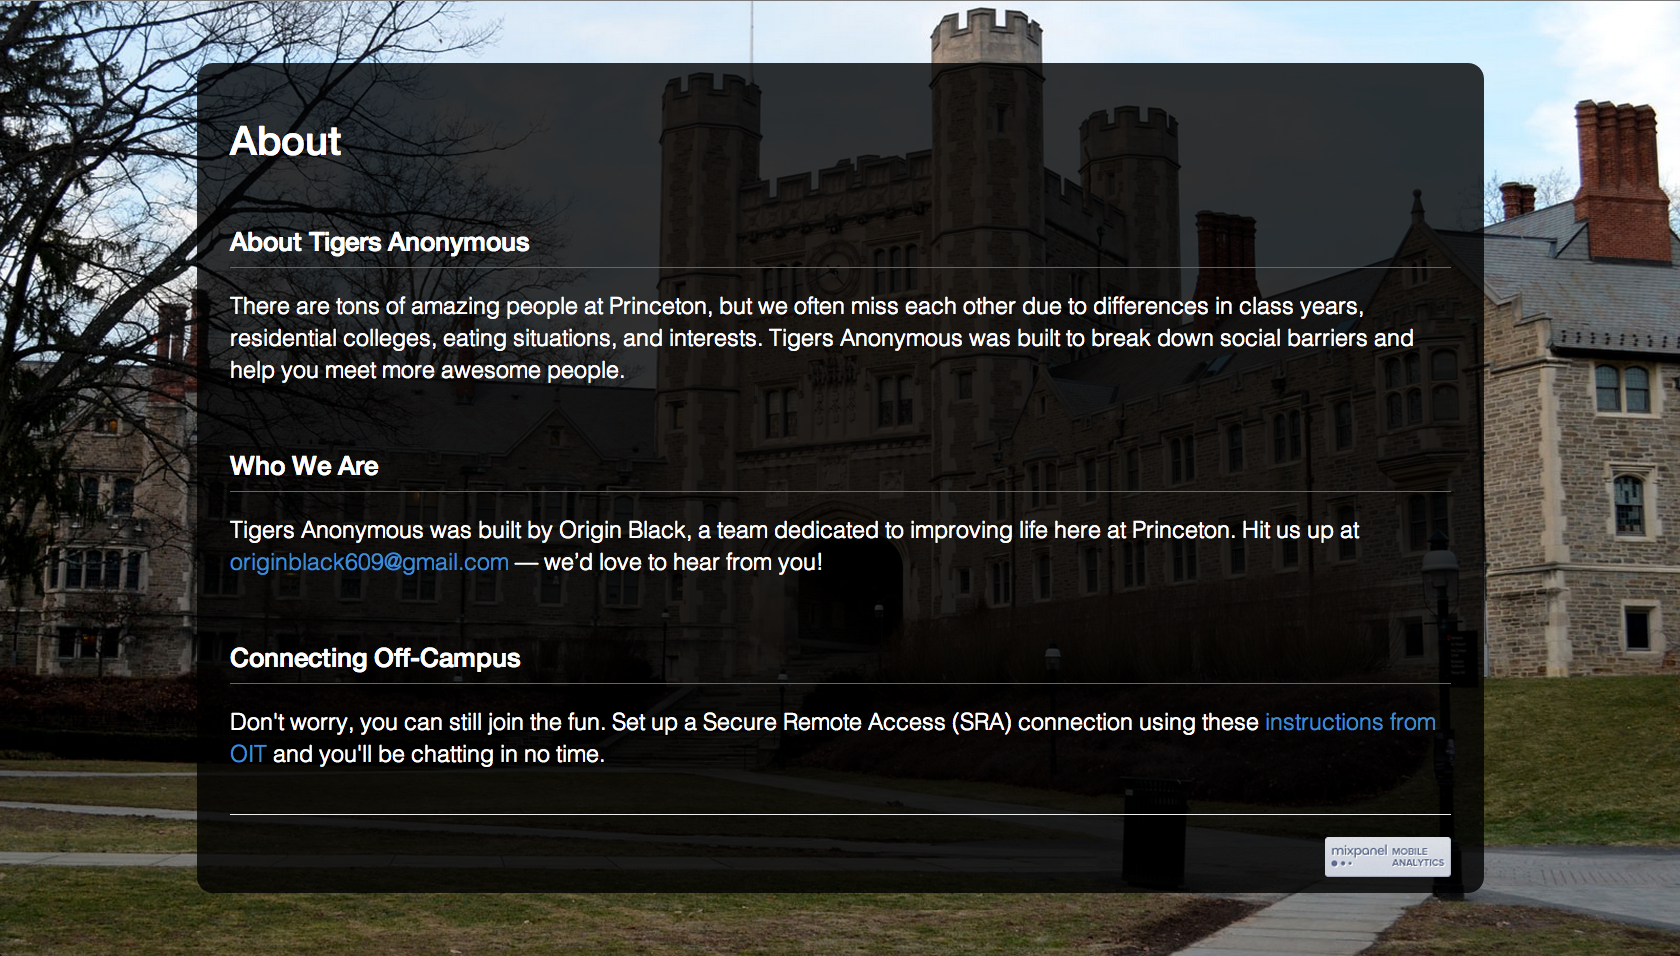
\includegraphics[trim= 35mm 0mm 35mm 0mm, clip, scale=0.25]{./Figures/TAAbout}
\caption{Tigers Anonymous About Page}
\label{fig:TAAbout}
\end{figure}

\lstset{language=HTML}
\begin{lstlisting}
<!DOCTYPE html>
<html>
  <head>
    <title>About - Tigers Anonymous</title>
    <link rel="icon" href="img/favicon.ico" type="image/x-icon">
    <meta name="viewport" content="width=device-width, initial-scale=1.0, user-scalable=no">
    <link rel="stylesheet" href="//netdna.bootstrapcdn.com/bootstrap/3.0.3/css/bootstrap.min.css">
    <link href="css/index.css" rel="stylesheet" type="text/css" media="all">
    <script>
      (function(i,s,o,g,r,a,m){i['GoogleAnalyticsObject']=r;i[r]=i[r]||function(){
      (i[r].q=i[r].q||[]).push(arguments)},i[r].l=1*new Date();a=s.createElement(o),
      m=s.getElementsByTagName(o)[0];a.async=1;a.src=g;m.parentNode.insertBefore(a,m)
      })(window,document,'script','//www.google-analytics.com/analytics.js','ga');
      ga('create', 'UA-23357698-2', 'tigersanonymous.com');
      ga('send', 'pageview');
    </script>
  </head>
  <body class="cover">
    <div class="wrapper">
      <div class="container">
        <div class="row">
          <div class="col-md-12">
            <h1>About</h1>
            <div class="header" id="about">
              <h3>About Tigers Anonymous</h3>
            </div>
            <p class="lead">
            There are tons of amazing people at Princeton, but we often miss each other due to differences in class years, residential colleges, eating situations, and interests. Tigers Anonymous was built to break down social barriers and help you meet more awesome people.
            </p>
            <div class="header" id="whoweare">
              <h3>Who We Are</h3>
            </div>
            <p class="lead">
            Tigers Anonymous was built by Origin Black, a team dedicated to improving life here at Princeton. Hit us up at <a href="mailto:originblack609@gmail.com">originblack609@gmail.com</a> &#8212 we�d love to hear from you!
            </p>
            <div class="header" id="offcampus">
              <h3>Connecting Off-Campus</h3>
            </div>
            <p class="lead">
            Don't worry, you can still join the fun. Set up a Secure Remote Access (SRA) connection using these <a href="http://helpdesk.princeton.edu/kb/display.plx?ID=6023">instructions from OIT</a> and you'll be chatting in no time.
            </p>
          </div>
        </div>
        <div class="row">
          <div class="col-md-12 text-right">
            <hr>
            <a href="https://mixpanel.com/f/partner"><img src="//cdn.mxpnl.com/site_media/images/partner/badge_light.png" alt="Mobile Analytics" /></a>
          </div>
        </div>
      </div>
    </div>
  </body>
</html>

\end{lstlisting}

\section{Chatroom}

The Tigers Anonymous chatroom (shown below in \ref{fig:TAChatRoom}) is implemented with the code shown at the bottom of this section.

\begin{figure}[h]
\centering
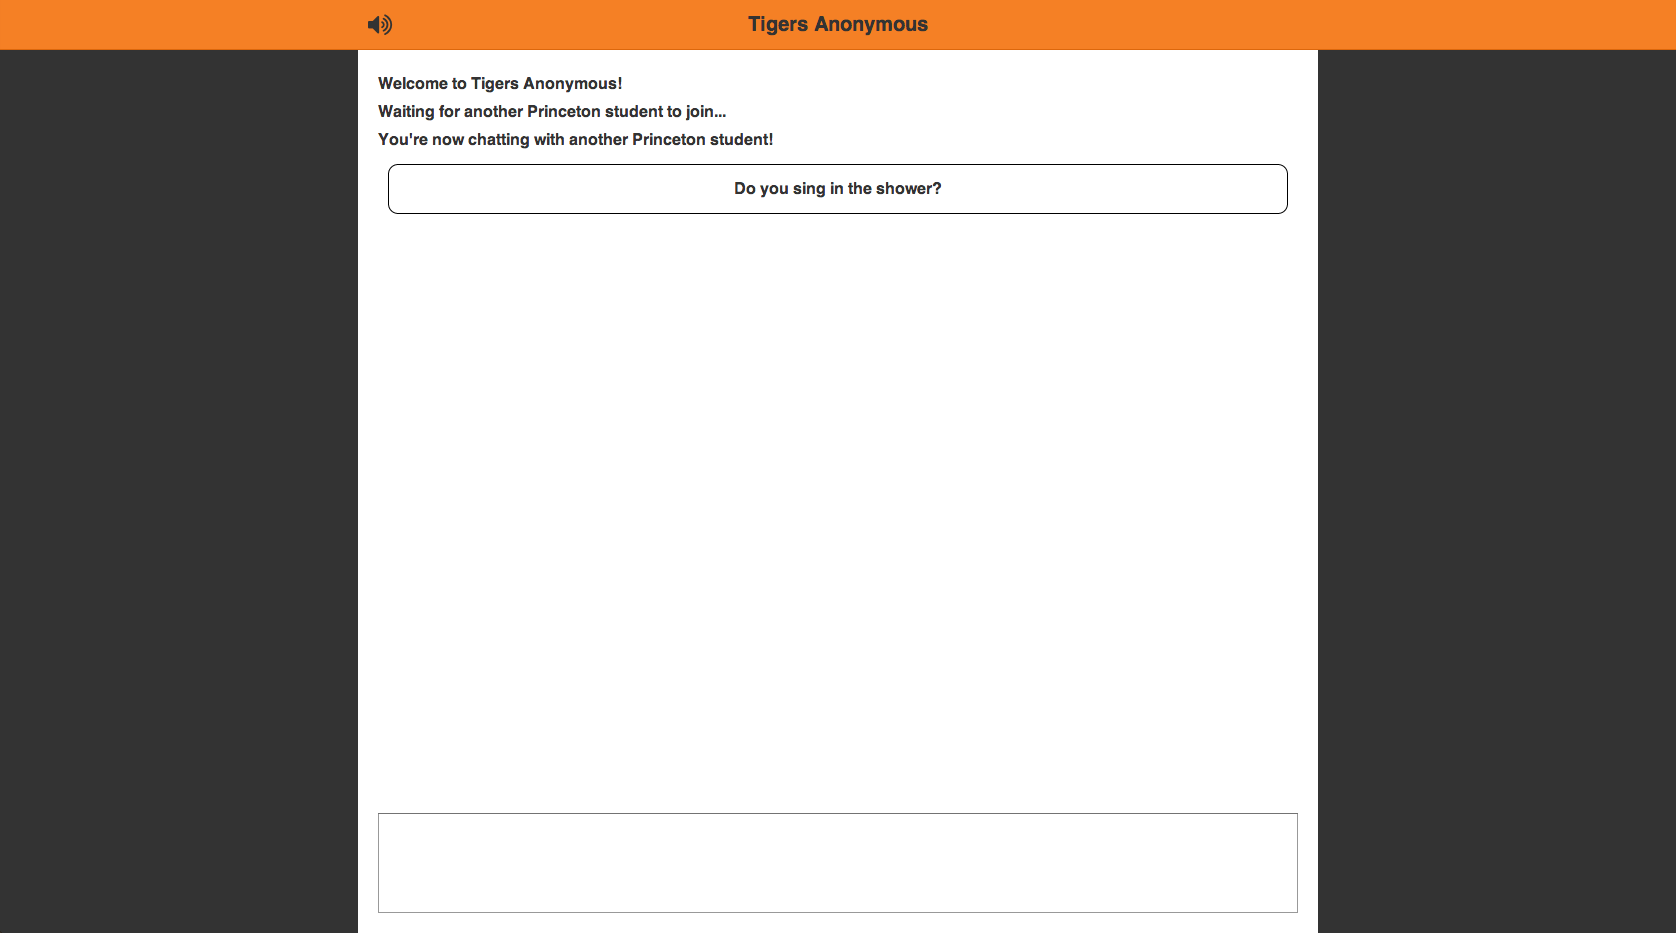
\includegraphics[trim= 35mm 0mm 35mm 0mm, clip, scale=0.25]{./Figures/TAChatroom}
\caption{Tigers Anonymous Chatroom}
\label{fig:TAChatRoom}
\end{figure}

\lstset{language=HTML}
\begin{lstlisting}

<!DOCTYPE html>
<html ng-app="pom">
  <head ng-controller="TitleCtrl">
    <title ng-bind="getTitle()">Tigers Anonymous</title>
    <link rel="icon" href="img/favicon.ico" type="image/x-icon">
    <meta name="viewport" content="width=device-width, initial-scale=1.0, user-scalable=no">
    <meta name="apple-mobile-web-app-capable" content="yes">
    <link href="//netdna.bootstrapcdn.com/font-awesome/4.0.3/css/font-awesome.css" rel="stylesheet">
    <link href="css/chat.css" rel="stylesheet" type="text/css" media="all">
  </head>
  <body ng-controller="ChatCtrl">
    <div id="fb-root"></div>
    <div class="nav">
      <div class="nav-container">
        <span class="brand" href="/">Tigers Anonymous</span>
        <a class="volume" ng-click="playSound = !playSound" ng-cloak>
          <i class="fa fa-volume-up" ng-show="playSound"></i>
          <i class="fa fa-volume-off" ng-show="!playSound"></i>
        </a>
        <a class="circle-down" ng-show="dropdown.shouldShowMinimized() && state == 'chatting'" ng-click="dropdown.show()" ng-cloak>
          <i class="fa fa-chevron-circle-down"></i>
        </a>
      </div>
    </div>
    <div class="chat-container">
      <div class="dropdown" ng-show="dropdown.shouldShowFull() && state == 'chatting'" ng-cloak>
        <div class="question">
          Do you want to find out who you've been chatting with?<br>
          <span class="promise">We'll never post to Facebook without your permission. Promise.</span>
        </div>
        <div class="options">
          <button type="button" class="yes-btn" ng-click="dropdown.accept()">Yes</button>
          <button type="button" class="hide-btn" ng-click="dropdown.hide()">Hide</button>
        </div>
      </div>
      <div class="chatroom" pom-scroll-glue>
        <ul ng-cloak>
          <li ng-repeat="message in messages" ng-class="message.type" ng-switch="message.type">
            <div ng-switch-when="chat">
              <span ng-class="{userName: !message.isPartner, partnerName: message.isPartner}">{{message.name}}:</span>
              <span ng-bind-html="message.text | linky | linkyNewlines"></span>
            </div>
            <div ng-switch-when="system">
              <div ng-switch="message.template" ng-class="{important: message.important}">
                <div ng-switch-when="entrance">
                  Welcome to Tigers Anonymous!
                </div>
                <div ng-switch-when="waiting">
                  Waiting for another Princeton student to join...
                </div>
                <div ng-switch-when="matched">
                  You're now chatting with another Princeton student!<br>
                  <div class="question-box">
                    {{message.question}}
                  </div>
                </div>
                <div ng-switch-when="selfRevealed">
                  Your partner's identity will be revealed if they also want to discover yours.
                </div>
                <div ng-switch-when="partnerRevealed">
                  Congratulations! You get to find out your partner's identity!<br>
                  You've been chatting with: <a href="{{message.partnerLink}}" target="_blank">{{message.partnerName}}</a>
                </div>
                <div ng-switch-when="fbError">
                  Sorry, there was an error connecting to Facebook. Please try again.
                </div>
                <div ng-switch-when="fbFake">
                  Sorry, it looks like you're using a fake Facebook account.
                </div>
                <div ng-switch-when="finished">
                  {{partnerName}} has disconnected. Refresh the page to start another chat!<br>
                  What do you think about Tigers Anonymous? <a href="https://docs.google.com/forms/d/1NI2nuAoYRZzYcawLrbWPKHsc43EdvbS5mU5d0A4cM2U/viewform" target="_blank">Let us know!</a>
                </div>
                <div ng-switch-when="disconnected">
                  You have been disconnected.
                </div>
                <div ng-switch-when="error">
                  Sorry, we're unable to connect you. Please check the following:
                  <ol>
                    <li>
                    You need to be using a computer connected to Princeton's network.<br>
                    If you're off-campus, <a href="about#offcampus">follow these instructions.</a>
                    </li>
                    <li>You can't already be chatting with a user.</li>
                    <li>You need to be using a modern web browser that supports WebSockets.</li>
                  </ol>
                </div>
                <div ng-switch-default>
                  {{message.text}}
                </div>
              </div>
            </div>
          </li>
          <li class="typing" ng-show="partnerTyping && state == 'chatting'">
            {{partnerName}} is typing...
        </ul>
      </div>
      <div class="input-wrapper">
        <textarea
          tabindex="1"
          pom-focus-on-chat
          ng-disabled="state != 'chatting'"
          ng-model="message"
          ng-keydown="sendMessage($event)"
          ng-change="updateTyping()"></textarea>
      </div>
    </div>
    <audio pom-play-on-message src="audio/notification.wav"></audio>
    <script src="/socket.io.js"></script>
    <script src="//ajax.googleapis.com/ajax/libs/angularjs/1.2.6/angular.min.js"></script>
    <script src="//ajax.googleapis.com/ajax/libs/angularjs/1.2.6/angular-sanitize.js"></script>
    <script src="//ajax.googleapis.com/ajax/libs/angularjs/1.2.6/angular-animate.js"></script>
    <!-- build:js js/app.js -->
    <script src="js/app.js"></script>
    <script src="js/controllers.js"></script>
    <script src="js/directives.js"></script>
    <script src="js/services.js"></script>
    <script src="js/filters.js"></script>
    <!-- endbuild -->
  </body>
</html>

\end{lstlisting}
